%! Author = danielmendes
%! Date = 15.02.25

\chapter{Partitionen}\label{ch:partitions}

In diesem Kapitel analysieren wir die Funktionsweise von Partitionen und das Verhalten des Abfrageoptimierers.
Zudem betrachten wir deren Verwendungszweck sowie die verschiedenen Typen, darunter RANGE-, LIST-, HASH- und KEY-Partitionierung\@.
Abschließend führen wir Benchmark-Tests durch, um die jeweiligen Vor- und Nachteile zu bewerten.

\section{Grundlagen}\label{sec:partition-grundlagen}

Bevor wir uns mit den verschiedenen Partitionierungstypen und deren Einsatzmöglichkeiten befassen, müssen wir klären, was eine Partition ist.
Eine partitionierte Tabelle ist eine logische Einheit, die aus mehreren physischen Subtabellen besteht (\cite[pp. 265--273]{schwartz2012high}).
Das System verwaltet die Partitionen intern, sodass der Benutzer nicht bemerkt, wie genau die Daten organisiert sind.
Dadurch wirken sie für ihn wie eine Blackbox.
Damit eine Tabelle die Partitionierung nutzt, muss bei ihrer Erstellung die \texttt{PARTITION BY}-Klausel angegeben werden, die festlegt, in welcher Partition jede Datenzeile gespeichert wird.
Dies führt zu einer erhöhten Komplexität der \texttt{CREATE TABLE}- und \texttt{ALTER TABLE}-Befehle.
In der Partitionsklausel selbst können nicht nur Ausdrücke und Berechnungen zur Bestimmung der Partitionierung eingesetzt werden, sondern auch Funktionen.
Die Funktionen müssen dazu jedoch eine nicht-konstante und deterministische Ganzzahl zurückgeben, wie z.B. \texttt{YEAR()}.
Wir werden gleich sehen, wie man erkennen kann, welche Komponenten-Tabellen intern verwendet werden.
% TODO(Daniel): dieser part hier gefällt mir nicht.
Bevor wir zu den Vorteilen der Partitionierung und deren Funktionsweise kommen, klären wir noch die Einschränkungen.
Zum einen müssen alle Spalten, nach denen die Partitionierung erfolgt, im Primärschlüssel oder Unique-Index enthalten sein.
Andernfalls ist es nicht möglich, die Partitionen korrekt zu erstellen oder zu verwalten.
Als logische Schlussfolgerung ergibt sich ein zusätzlicher Aufwand für die Pflege der neuen Indizes.
Außerdem können keine Fremdschlüssel-Bedingungen (engl.\ foreign key constraints) verwendet werden.
Darüber hinaus gibt es ein Limit für die Anzahl der Partitionen pro Tabelle.
Bei älteren MySQL-Versionen liegt dieses Limit bei 1024 und seit MySQL-Version 8.0 bei 8192 Partitionen (\cite{mysql_nof_partitions}).
Wie wir später noch feststellen werden, sollte aus verschiedenen Gründen die Anzahl der Partitionen so gering wie möglich gehalten werden.
Aus diesem Grund ist diese Einschränkung nicht sehr relevant, sollte aber im Hinterkopf behalten werden.

Da wir die Bedingungen nun geklärt haben, kommen wir als Nächstes zu der Funktionsweise.
Wie bereits erwähnt, bestehen partitionierte Tabellen aus mehreren zugrunde liegenden Tabellen, die durch Handler-Objekte verwaltet werden.
% TODO(Daniel): dieser part hier gefällt mir nicht.
Ein Handler-Objekt dient als Schnittstelle für den Zugriff auf die Daten einer Partition und ermöglicht MySQL, die zugrunde liegenden Tabellen so zu nutzen, als wären sie eigenständige Tabellen.
Aus Sicht der Storage Engine sind Partitionen einfach Tabellen, unabhängig davon, ob sie eigenständig oder Teil einer partitionierten Tabelle sind.
Jede Partition wird von der Storage Engine auf übliche Weise verwaltet, jedoch können die einzelnen Partitionen nicht immer direkt angesprochen werden.
Das hängt jedoch auch vom jeweiligen Datenbankmanagementsystem ab.
In Oracle ist dies wie folgt möglich:

\vspace{-5pt}
\begin{lstlisting}[language=SQL,label={lst:direct_partition}]
SELECT * FROM your_table PARTITION (your_partition_name);
\end{lstlisting}
\vspace{-7pt}

Bei der Partitionierung in MySQL werden Indizes für jede Partition separat definiert, anstatt sie über die gesamte Tabelle hinweg zu erstellen.
Alle Indexe der Tabelle werden dabei als identische Indexe auf jede Partition angewendet.
Die genaue Implementierung hängt jedoch vom jeweiligen DBMS ab und kann variieren.
Beispielsweise in Oracle können Indexe und Tabellen auf flexiblere und komplexere Weise partitioniert werden.

Als Nächstes gilt es zu verstehen, wann und wie die Partitionierung zu Performancegewinnen führen kann.
Der Abfrageoptimierer (engl.\ Query Optimizer) versucht, beim Ausführen von Abfragen Partitionen auszuschließen und nur die relevanten Partitionen zu durchsuchen, die die gesuchten Daten enthalten.
Dies geschieht immer dann, wenn eine \texttt{WHERE}-Klausel mit dem Partitionsausdruck übereinstimmt.
Der Fachbegriff dafür heißt Pruning.
Bei SELECT-Abfragen entscheidet der Query-Optimizer, ob bestimmte Partitionen ignoriert werden können und leitet die Anfragen an die Storage Engine weiter.
Bei INSERT-Abfragen wird bestimmt, welche Partition die neue Zeile erhält und der Befehl wird dementsprechend übergeben.
Ähnlich funktioniert es bei DELETE-Abfragen, bei denen die Löschanfrage an die passende Partition weitergegeben wird.
Man sollte sich auch in Erinnerung rufen, dass beim Löschen einer Zeile diese zuerst lokalisiert werden muss.
Bei UPDATE-Abfragen innerhalb einer Partition wird die Anfrage ebenfalls an die jeweilige Partition übermittelt.
Wenn aber Teile der Partitionslogik verändert werden, dann stellt UPDATE eine Kombination von INSERT und DELETE dar, da eine Einfügungsanfrage an die Zielpartition und eine Löschanfrage an die Quellpartition weitergeleitet wird.
Die meisten dieser Operationen unterstützen Pruning, einige, wie z.B.\ INSERT-Abfragen, sind von Natur aus ausschließend (engl.\ self-pruned).

In der Funktionsweise des Pruning kann man auch den Hauptzweck der Partitionierung erkennen, denn wie bei der Indexierung und der Datenclusterung einer Tabelle, trägt es dazu bei, große Teile der Tabelle vom Zugriff auszuschließen und zusammengehörige Zeilen nahe beieinander zu speichern.
Statt Indexe zu verwenden, bietet es sich an Tabellen ohne Indexe zu erstellen und ausschließlich die Partitionierung zu nutzen, um gezielt auf die gewünschten Zeilen zuzugreifen.
Wenn man sich in der Nähe der gewünschten Daten befindet, kann man von dort aus entweder das relevante Datengebiet sequentiell scannen oder es in den Speicher laden und indexieren.
Zudem hat die Partitionierung einen geringen Mehraufwand, weil es keine Datenstruktur gibt, die auf einzelne Zeilen zeigt und ständig aktualisiert werden muss.
Sie lassen sich auch physisch verteilen, sodass der Server mehrere Festplatten effizienter nutzen kann.
Darüber hinaus erfolgt die Identifikation der Daten nicht auf Zeilenebene und es wird keine separate Datenstruktur verwendet.
Stattdessen gibt es eine mathematische Formel, die bestimmt, welche Partitionen welche Kategorien von Zeilen enthalten können.
Wenn wir Partitionen anstelle von Indizes verwenden, steigt die Effizienz, je mehr Partitionen durch die WHERE-Klausel in der Abfrage ausgeschlossen werden.
Besonders vorteilhaft können Partitionen sein, wenn die Tabellen sehr groß sind und nicht mehr vollständig in den Speicher passen.
Außerdem sind partitionierte Daten einfacher zu verwalten, da gesamte Partitionen gelöscht oder auch wiederhergestellt werden können.

Die Effizienz von Partitionierung basiert auf zwei wichtigen Annahmen.
Zum einen muss man die Suche durch das Pruning von Partitionen beim Abfragen eingrenzen können und zum anderen muss die Partitionierung selbst nicht sehr kostspielig sein.
Diese Annahmen sind aber nicht immer gültig.
Im Folgenden betrachten wir 3 unterschiedliche Anwendungsfälle, bei denen mögliche Fehler im Umgang mit Partitionen beschrieben werden.

Zuallererst kann das Ergebnis der Partitionsfunktion \texttt{NULL} sein.
Selbst wenn man die zeitbasierte Spalten als \texttt{NOT NULL} deklariert, können Werte gespeichert werden, die kein gültiges Datum sind.
Alle Zeilen, deren Datum entweder NULL oder nicht gültig ist, werden in MySQL in der ersten definierten Partition gespeichert.
Deshalb muss man bei einer Abfrage, die alle Jahre außer 2020 herausfiltert, anstelle einer Partition zwei Partitionen durchsuchen.
Die damit verbundenen Leistungsprobleme nehmen mit der Größe der ersten Partition zu.
Daher sollte man entweder eine dedizierte Partition für diese Sonderfälle einführen oder Funktionen wie \texttt{RANGE COLUMNS} verwenden.

Wenn man einen Index definiert, der nicht mit der Partitionsklausel übereinstimmt, können unerwartet mehr Partitionen durchsucht werden.
Man sollte daher versuchen, auf nicht partitionierten Spalten keine Indexe zu erstellen, es sei denn, die Abfragen enthalten einen Ausdruck, der beim Pruning der Partitionen hilft.
Manchmal lässt sich dieses Problem nicht auf den ersten Blick erkennen.
Angenommen eine partitionierte Tabelle ist die zweite Tabelle in einem Join und der Index, der für den Join verwendet wird, ist nicht Teil der Partitionsklausel, dann wird jede Zeile im Join jede Partition in der zweiten Tabelle durchsuchen.
% TODO(Daniel): dieser part hier gefällt mir nicht.
Bei der Range-Partitionierung kann die Bestimmung der korrekten Partition teuer sein, weil der Server die Liste der Partitionsdefinitionen durchsucht, um die Richtige zu finden.
Diese lineare Suche ist nicht sehr effizient und es steigen die Kosten, je mehr Partitionen es gibt.
Das Öffnen und Sperren von Partitionen, wenn eine Abfrage auf eine partitionierte Tabelle zugreift, ist eine andere Art von Overhead pro Partition.
Sie erfolgt vor dem Pruning, sodass dieser Overhead nicht pruned werden kann.
Außerdem ist diese Art von Overhead unabhängig vom Partitionierungstyp und betrifft alle Arten von Anweisungen.
Deshalb besagt der dritte Leitsatz, dass die Anzahl der definierten Partitionen begrenzt werden sollte.

Alle Partitionen sollten dieselbe Storage Engine nutzen, was Einschränkungen bei den verwendbaren Funktionen und Ausdrücken mit sich bringt.
Zudem unterstützen einige Storage Engines keine Partitionierung.

\section{Arten der Partitionierung}\label{sec:arten-der-partitionierung}

In diesem Unterkapitel werden wir die verschiedenen Partitionierungsarten, die von MySQL unterstützt werden, jeweils mit einem Beispiel näher erläutern.
Die Analyse der Ergebnisse erfolgt in Abschnitt~\ref{sec:partition-analyse}.
Als Grundlage verwenden wir die Kundentabelle (\ref{lst:tools-create-table-kunde}) und die Bestelltabelle (\ref{lst:tools-create-table-bestellung}), die bereits in früheren Kapiteln zum Einsatz kamen.
Die Tabelle, die wir auf unterschiedliche Partitionen verteilen wollen, ist die Kundentabelle.
Allerdings müssen wir beide Tabellen noch etwas anpassen, da es einige Einschränkungen für die partitionierte Tabellen gibt.
Zum einen muss bei der Bestelltabelle bei allen Typen die Fremdschlüssel-Bedingung entfernt werden und zum anderen muss der Primärschlüssel der Kundentabelle angepasst werden.
Wie genau das passieren muss, werden wir an den Beispielen erkennen.
Die Insert-Befehle sind bei allen Typen der Partitionierung gleich, bei den Select-Queries gibt es jedoch Unterschiede.

Den ersten Typ, den wir betrachten, ist die RANGE-Partitionierung.
Bei dieser erfolgt die Zuordnung von Zeilen zu Partitionen basierend auf Spaltenwerten, die in einen definierten Wertebereich fallen.
Für unser Beispiel wollen wir unterschiedliche Partitionen je nach Alter des Kunden.
Alle fünf Jahre soll es eine neue Partition geben.

\vspace{-8pt}
\lstinputlisting[
	language=sql,
	caption=Kundetabelle mit Range-Partitionierung,
	label={lst:create_kunden_partition_range},
	style=custom_daniel,
]{Scripts/Partition/01_Create_Kunden_Partition_Range.sql}
\vspace{-5pt}

Damit es zu keinen Fehlern kommt, muss hier der Geburtstag auch Teil des Primärschlüssels der Kundentabelle sein.
Außerdem muss die Spalte \texttt{GEBURTSTAG} bei der Bestelltabelle hinzugefügt werden, damit das Joinen der Tabellen über den Primärschlüssel effizienter ist.
Seit MySQL 5.5 kann für Datumsspalten auch der Partitionierungstyp \texttt{RANGE COLUMNS} verwendet werden, wodurch bei der Partitionsklausel die Funktion \texttt{YEAR()} nicht erforderlich ist.

Um die Performance der beiden Ansätze zu vergleichen, verwenden wir beide Varianten bei der Tabellenerstellung.
Bei der Range-Partitionierung testen wir mehrere Select-Befehle, da je nach Art der Abfrage des Datums das Pruning besser oder schlechter funktioniert (siehe Abschnitt~\ref{sec:partition-grundlagen}).
Dazu joinen wir zunächst die Kundentabelle an die Bestelltabelle über die Attribute \texttt{KUNDEN\_ID} und \texttt{GEBURTSTAG}.
Die Testkunden werden so generiert, dass sie immer zufällig zwischen den Jahren 1950 und 2020 geboren sind.
Die darauffolgenden \texttt{WHERE}-Bedingungen unterscheiden sich aber zwischen den unterschiedlichen Select-Befehlen.

\vspace{-5pt}
\begin{lstlisting}[language=SQL,caption=Unterschiedliche WHERE-Bedingungen,label={lst:different_where_conditions}]
WHERE YEAR(k.GEBURTSTAG) = 1985;		             -- failing_pruning.sql
WHERE k.GEBURTSTAG BETWEEN '1985-01-01' AND '1985-12-31'; 	-- with_pruning.sql
WHERE k.GEBURTSTAG = '1985-01-01';		            -- with_primary_key.sql
\end{lstlisting}
\vspace{-5pt}

Bevor wir die Performance dieser Abfragen analysieren, wollen wir überprüfen, ob der Optimierer die Partitionen pruned oder nicht.
Dazu kann man SQL-Befehl \texttt{EXPLAIN} vor dem \texttt{SELECT}-Befehl in~\ref{lst:different_where_conditions} nutzen.
Als Rückgabe erhält man eine Übersicht, wie MySQL die Abfrage ausführt und welche Partitionen verwendet wurden.
Zunächst führen wir Query aus, bei der wir keine \texttt{WHERE}-Klausel angeben.
Im Ergebnis von \texttt{EXPLAIN} sehen wir, dass der Abfragemechanismus alle Partitionen durchsuchen muss, was bei großen Tabellen die Performance stark beeinträchtigen kann.
Bei der \texttt{WHERE}-Klausel der Abfrage in Zeile 1 würden wir erwarten, dass nur eine Partition abgefragt wird, aber wir erhalten das gleiche Resultat wie bei der Abfrage davor.
Die Query aus der zweiten Zeile verweist direkt auf die Partitionsspalte und nicht auf einen Ausdruck.
Und tatsächlich wird, wie erwartet, nur die Partition zwischen den Jahren 1985 und 1990 untersucht.
Diese Partition wir auch as einzige bei der Abfrage aus der letzten Zeile benutzt.
Daraus lässt sich schließen, dass MySQL nur dann Partitionen effizient prunen kann, wenn die Abfrage direkt auf die Partitionsspalte zugreift und keine Ausdrücke verwendet.
Man kann dieses Verhalten mit dem von indexierten Spalten vergleichen, die auch im Abfrageausdruck isoliert sein müssen, damit der Index verwendet werden kann.

Als Nächstes betrachten wir die LIST-Partitionierung, bei der die Partitionen anhand von Spaltenwerten ausgewählt werden, die einem der vordefinierten diskreten Werte entsprechen.
Zur Veranschaulichung möchten wir pro Land eine eigene Partition erstellen.
Dafür muss die Spalte \texttt{LAND} Teil des Primärschlüssels sein.
Beim Einfügen der Testdaten wählen wir pro Kunde ein zufälliges Land aus der Liste der 20 einwohnerreichsten Länder der Welt aus.
Damit müssen wir bei der Erstellung der Tabelle auch 20 Partitionen sowie eine Zusätzliche für sonstige Werte erstellen (\ref{lst:create_kunden_partition_list}).

\vspace{-5pt}
\lstinputlisting[
	language=sql,
	caption=Kundetabelle mit List-Partitionierung,
	label={lst:create_kunden_partition_list},
	style=custom_daniel,
]{Scripts/Partition/02_Create_Kunden_Partition_List.sql}
\vspace{-5pt}

Auch bei der List-Partitionierung wird die Performance von unterschiedlichen Select-Befehlen überprüft.
Zunächst joinen wir, wie zuvor, die Kundentabelle mit der Bestelltabelle und in der WHERE-Bedingung filtern wir so, dass alle Kunden aus Deutschland kommen.
Genau die gleiche Query verwenden wir beim Vergleich mit der Referenz ohne Partition.
Zusätzlich wollen wir die Performance untersuchen, wenn aus der Liste an Ländern zufällig fünf ausgewählt werden und alle Kunden nur aus einem dieser fünf Ländern kommen.
Dazu testen wir 3 verschiedene Ansätze.
Zum einen über den \texttt{OR}-Operator, den anderen mithilfe des \texttt{IN}-Operators und als letztes fragen wir die 5 Länder, wie im ersten Beispiel, einzeln ab und verbinden die Ergebnisse der 5 Antworten mithilfe des \texttt{UNION}-Operators.
Mithilfe von \texttt{EXPLAIN} wird sichtbar, dass bei allen Varianten nur die Partitionen der 5 Länder genutzt werden.
Damit kann der Optimierer Bereiche in Listen diskreter Werte umwandeln, Elemente prunen und während der Abfrageverarbeitung Partitionen gezielt entfernen.
Im Zusammenhang mit Joins ist der Effekt besonders stark, da MySQL bei einem partitionierten Schlüssel in der Join-Bedingung nur in den relevanten Partitionen nach übereinstimmenden Zeilen sucht.
Welche der Varianten aber am effizientesten ist, werden wir erst bei der Analyse sehen.

Zum Schluss betrachten wir die HASH-Partitionierung, bei der die Partition anhand eines Hash-Werts zugewiesen wird, der aus den Spaltenwerten der Zeilen berechnet wird.
Dazu müssen wir nur wenig verändern und aussschließlich die Zeilen aus dem Codeblock~\ref{lst:create_kunden_partition_hash} am Ende des Create Kunden-Befehls hinzufügen.
In diesem Fall testen wir auch nur eine einzige Select-Query, die wieder beide Tabellen joined und in der \texttt{WHERE}-Bedingung überprüft, ob die \texttt{KUNDEN\_ID} zwischen den Werten 1000 und 2000 liegt.
Damit wir mehr Werte miteinander vergleichen können, testen wir verschiedene Varianten der Hash-Partitionierung, indem wir die Anzahl der Partitionen variieren.
Die Anzahl der Partitionen beträgt in unseren Benchmarks 5, 50 und 500.
Einschließlich des Referenzfalls ergeben sich somit vier unterschiedliche Testfälle, die wir miteinander vergleichen.

\vspace{-5pt}
\begin{lstlisting}[language=SQL,caption=Hash-Partitonierung,label={lst:create_kunden_partition_hash}]
PARTITION BY HASH(KUNDEN_ID)
PARTITIONS 5;
\end{lstlisting}
\vspace{-5pt}

Die KEY-Partitionierung ähnelt der Hash-Partitionierung, verwendet jedoch die interne Hash-Funktion von MySQL und benötigt nur die Angabe einer oder mehrerer Spalten.
Um die Performance zu überprüfen, machen wir genau das Gleiche wie bei der Hash-Partitionierung.
Dafür müssen wir nur im Codeblock~\ref{lst:create_kunden_partition_hash} das Signalwort \texttt{HASH} mit \texttt{KEY} ersetzen und stellen das Ergebnis mit dem von \texttt{HASH} gegenüber.
Die Erkenntnisse aus diesem Benchmark schließen wir im nächsten Kapitel.

\section{Analyse}\label{sec:partition-analyse}

Im vorherigen Abschnitt wurden die verschiedenen Arten von Partitionen erläutert.
Nun möchten wir für jedes dieser Beispiele Benchmarks durchführen und die Ergebnisse untersuchen.
Um den Einfluss der Partitionierung auf die Abfragen zu verdeutlichen, vergleichen wir jeweils partitionierte mit nicht partitionierten Tabellen.
Beide Varianten stellen die gleichen Insert-Befehle, während sich die Select-Queries je nach Partitionierungstyp leicht unterscheiden können.
Abhängig vom Typen stellen wir zusätzlich leicht unterschiedliche Abfragen.
Die Ergebnisse des Referenzbenchmarks sollten weitgehend mit denen der partitionierten Varianten übereinstimmen.
Es kann aber kleinere Unterschiede geben, da wir jeweils zufällige generierte Daten einfügen.
Bei signifikanten Abweichungen sind die Performancemessungen jedoch schwerer miteinander vergleichbar.

Im ersten Benchmark mit der Range-Partitionierung fällt auf, dass die Benutzung von \texttt{RANGE} oder \texttt{RANGE COLUMNS} keinerlei Einfluss auf die Performance hat.
Daher stellt sich bei der Verwendung nicht die Frage nach der Performance, sondern nur welche Art der Definition der Nutzer bevorzugt.
Wenn wir die Abbildung~\ref{fig:range-partition} analysieren, dann wird klar, dass die \texttt{with\_pruning}-Query mit deutlichem Abstand schneller ist als die anderen.
Damit funktioniert das Pruning besonders gut, wenn die Geburtstage zwischen dem ersten und letzten Tage des Jahres abfragen.
Als Nächstes kommen die Skripte ohne Partitionierung, die aber etwa 50\% ineffizienter sind, als das Skript zuvor.
Da beide auf einem sehr ähnlichen Niveau liegen, kann davon ausgehen, dass die Verarbeitung durch \texttt{YEAR()} hier keine Rolle spielt.
Etwas langsamer bei der Range-Partitionierung ist \texttt{with\_primary\_key}, bei der wir nur die Kunden erhalten, die am 1.\ Januar 1985 geboren wurden.
Wenn wir die Ergebnisse von \texttt{EXPLAIN} betrachten, dann sehen wir, dass bei der Abfrage nur eine Partition benutzt wurde.
Als Letztes kommen die beiden Select-Queries, die alle Partitionen durchsuchen.
Bei der einen haben wir keine \texttt{WHERE}-Bedingung angegeben und bei der anderen haben wir die Funktion \texttt{YEAR()} benutzt.
Es lässt sich also feststellen, dass Pruning mithilfe von \texttt{YEAR()} offensichtlich nicht funktioniert.
Dies bestätigt auch der Ausführungsplan für die Query.
Bei den Insert-Befehlen ist der Fall ohne Partitionierung nur geringfügig schneller als mit Partitionierung.

\vspace{-6pt}
\begin{figure}[H]
	\centering
	\begin{subfigure}[t]{0.48\textwidth}
		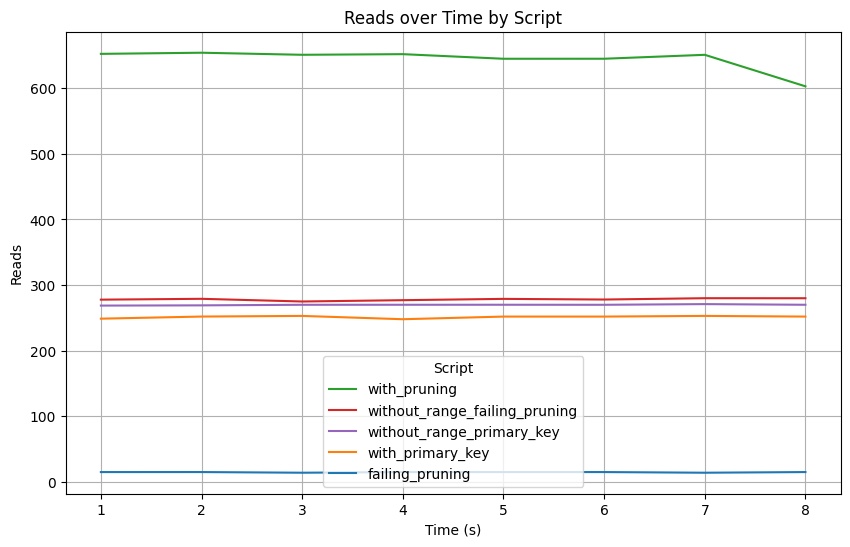
\includegraphics[width=\textwidth]{PNGs/Script/Partition/range-partition/Reads}
	\end{subfigure}
	\hfill
	\begin{subfigure}[t]{0.48\textwidth}
		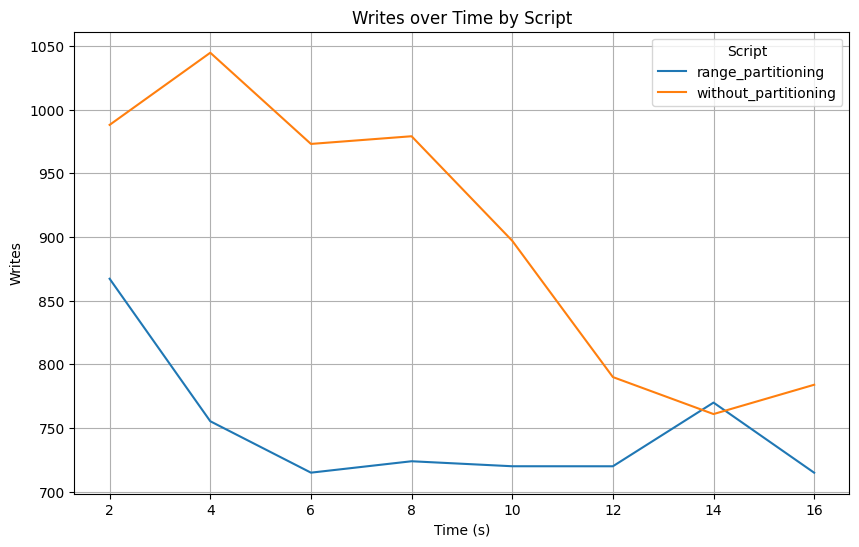
\includegraphics[width=\textwidth]{PNGs/Script/Partition/range-partition/Writes}
	\end{subfigure}
	\vspace{-8pt}
	\caption[Range-Partitionierung: Unterschiedliche Selects mit und ohne Partition]{Vergleich zwischen der Range-Partitionierung und ohne Partition}
	\label{fig:range-partition}
\end{figure}
\vspace{-19pt}

Bei der List-Partitionierung~\ref{fig:list-partition} können wir auch einige interessante Beobachtungen machen.
Beim ersten Fall ist nur ein Land in der WHERE-Bedingung vorhanden.
Wenn dies so ist, dann hat die Partitionierung einen erheblichen Vorteil gegenüber der Version ohne Partitionierung (siehe rote Linie von \texttt{with\_pruning\_simple} und braune von \texttt{without\_list\_pruning\_simple}).
Wenn wir statt nur eines Landes mehrere abfragen, sehen wir für die verschiedenen Operatoren unterschiedliche Ergebnisse.
Die beste Performance erzielt der IN-Operator.
Dicht darauf folgt der OR-Operator.
Mit etwas größerem Abstand liegt der Fall ohne Partitionierung.
Deutlich abgeschlagen ist die Verbindung der Ergebnisse per UNION-Operator.
Die Performance beim Einfügen der Daten ist bei der Partitionierung und dem Referenzfall sehr ähnlich, wobei letzterer einen ganz leichten Vorteil hat.

\vspace{-6pt}
\begin{figure}[H]
	\centering
	\begin{subfigure}[t]{0.48\textwidth}
		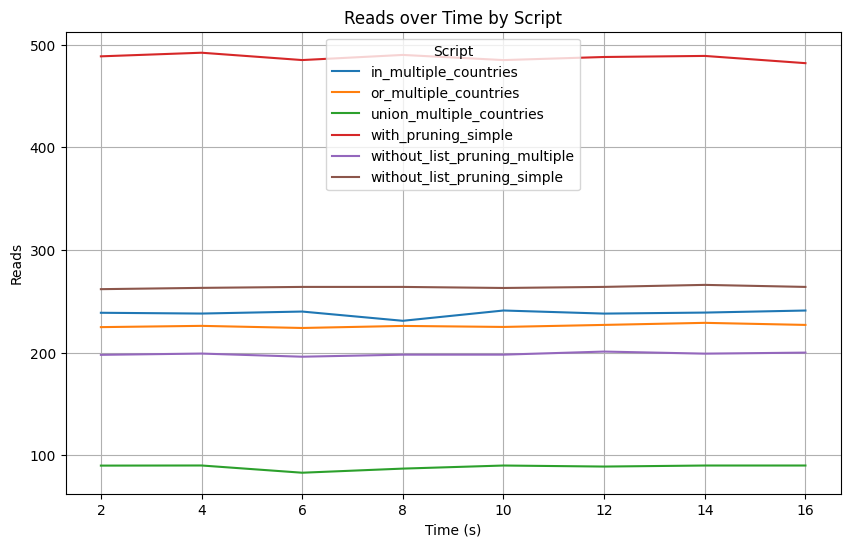
\includegraphics[width=\textwidth]{PNGs/Script/Partition/list-partition/Reads}
	\end{subfigure}
	\hfill
	\begin{subfigure}[t]{0.48\textwidth}
		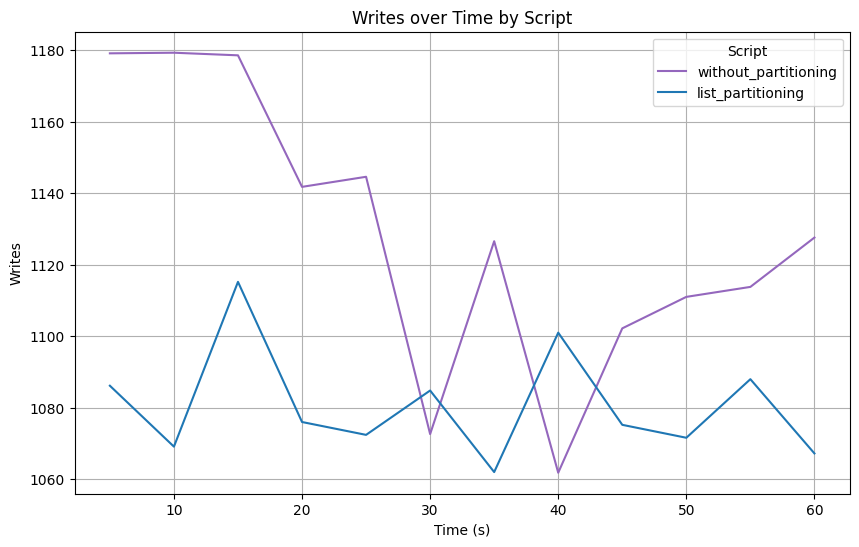
\includegraphics[width=\textwidth]{PNGs/Script/Partition/list-partition/Writes}
	\end{subfigure}
	\vspace{-8pt}
	\caption[List-Partitionierung: Unterschiedliche Abfragen mit und ohne Partition]{Vergleich zwischen der List-Partitionierung und ohne Partition}
	\label{fig:list-partition}
\end{figure}
\vspace{-19pt}

Bei der Key-Partitionierung fällt auf, dass es keinen signifikanten Performance-Unterschied zur Hash-Partitionierung gibt, wenn derselbe Datensatz und dieselbe Anzahl von Partitionen verwendet wird.
Generell ist die Key-Partitionierung häufig stabiler und optimierter ist, insbesondere wenn es um Primärschlüssel geht.
Bei der Hash-Partitionierung~\ref{fig:hash-partition} nehmen sich beide Select-Fälle kaum etwas.
Auch hier fällt auf, dass die Werte der Abfragen sehr konstant sind.
Nur bei der Variante mit 500 Partitionen gibt es deutlich sichtbare Schwankungen.
Diese liegen aber nicht an dem Pruning, denn mit dem SQL-Befehl \texttt{EXPLAIN} sehen wir, dass alle 500 Partitionen benötigt werden und nicht keine Partitionen durch Zufall geprunt werden.
Die Hash-Partitionierung berechnet aus dem Wert einer bestimmten Spalte mithilfe einer Hash-Funktion einen Hash-Wert und anhand dessen wird die Zeile einer der Partitionen zugewiesen.
Da der Hash-Wert bei 500 Partitionen mit modulo 500 gebildet wird, landet jeder 500-ste Wert in der gleichen Partition.
Damit ist klargestellt, dass immer alle Partitionen benutzt werden, was die folgenden Ergebnisse zeigen.
Zunächst zeigt sich, dass die Abfrage ohne Partitionierung am schnellsten ist.
Danach lässt sich die Regel ableiten, dass eine höhere Anzahl an Partitionen zu einer langsameren Abfrage führt.
Dies liegt daran, dass mehr Partitionen die Suche innerhalb der Struktur komplexer machen und dadurch die Performance beeinträchtigen.
Der Unterschied zwischen ohne Partitionen und 5 Partitionen ist noch überschaubar, aber bei 500 Partitionen sieht man einen sehr deutlichen Unterschied.

\vspace{-4pt}
\begin{figure}[H]
	\centering
	\begin{subfigure}[t]{0.48\textwidth}
		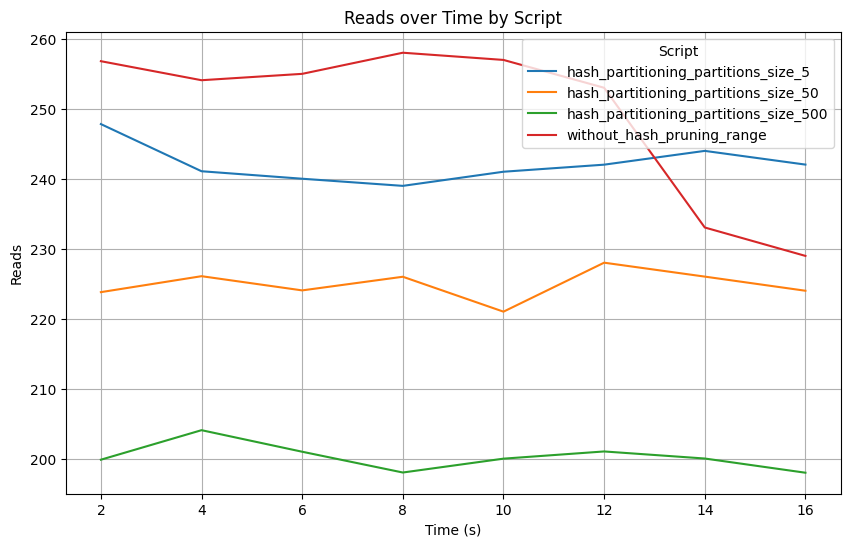
\includegraphics[width=\textwidth]{PNGs/Script/Partition/hash-partition/Reads}
	\end{subfigure}
	\hfill
	\begin{subfigure}[t]{0.48\textwidth}
		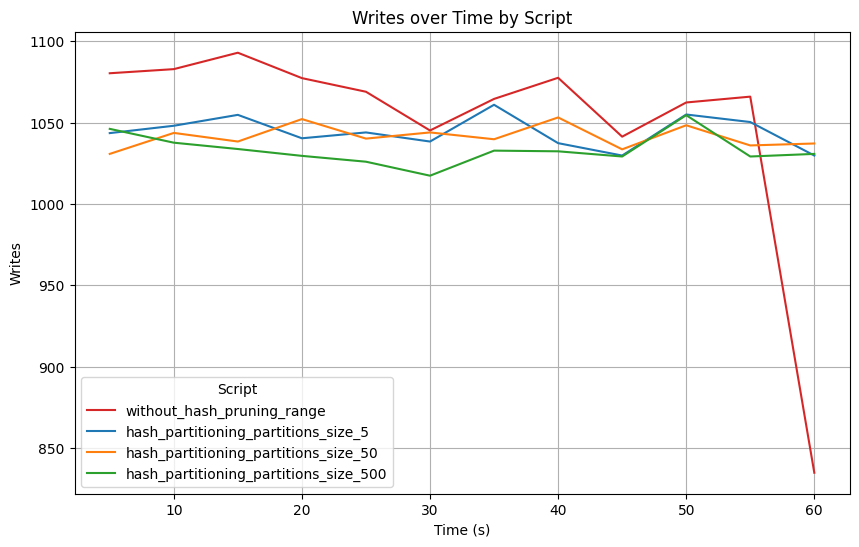
\includegraphics[width=\textwidth]{PNGs/Script/Partition/hash-partition/Writes}
	\end{subfigure}
	\vspace{-8pt}
	\caption[Hash-Partitionierung: Variationen der Partitionsanzahl]{Vergleich zwischen der Hash-Partitionierung und ohne Partition}
	\label{fig:hash-partition}
\end{figure}
\vspace{-12pt}